% Creating a simple Title Page in Beamer
\documentclass{beamer}

% Theme choice:
% \usetheme{CambridgeUS}
\usetheme{Singapore}
% \usetheme{JuanLesPins}
\usefonttheme{serif}
\usecolortheme{dolphin}
% \usecolortheme{spruce}
\usecolortheme{seagull}
% \usecolortheme{dove}
\setbeamertemplate{itemize items}[Madrid]
\setbeamertemplate{enumerate items}[Madrid]

%images
\usepackage{graphicx}
\graphicspath{ { ./presentation/ } }


% Title page details: 
\title{Decrypting Encryptions}
\author{Shubhro Gupta}
\date{\today}

\begin{document}

% Title page frame
\begin{frame}
	\titlepage
\end{frame}

\begin{frame}
	{Table of Contents}
	\tableofcontents
\end{frame}

\section{Encryption Basics}

\subsection{Introduction}
\begin{frame}
	\begin{itemize}
		\item Encryption is the process of converting information or data into a code, especially to prevent unauthorized access.
		\item Encryption helps protect data you send, receive, and store using any device.
		\item Encryption is a way to enhance the security of a message or file by scrambling the contents so that only someone with the right encryption key can unscramble it.
	\end{itemize}
\end{frame}

\subsection{Caesar Cipher}
\subsection{Substitution Cipher}


\section{Mathematics Basics}
\subsection{Modular Function}
\begin{frame}
	\begin{block}{Modular Function}
		Basically the remainder of a division operation.\\
	\end{block}
	$a \mod b = r$, where $r$ is the remainder when $a$ is divided by $b$.
\end{frame}


\subsection{Prime Numbers}
\begin{frame}
	\emph{Prime Numbers. }
	A $1 < n \in \mathbb{N}$ that is not a product of two smaller natural numbers.\\
	~\\

	\emph{Semiprime. }
	A $n \in \mathbb{N}$ that is the product of two prime numbers.\\
	~\\

	\emph{Coprime. }
	Two numbers are coprime if their greatest common divisor is 1.
\end{frame}


\subsection{Totient Function}

\begin{frame}
	\begin{block}{Euler's Totient Function}
		The totient function $\phi(n)$ is defined as the number of positive integers less than $n$ that are coprime to $n$.
	\end{block}

\end{frame}

\begin{frame}
	\begin{center}$\phi(8)$\end{center}
	\begin{align*}
		GCD(1, 8) & = 1 \\
		GCD(2, 8) & = 2 \\
		GCD(3, 8) & = 1 \\
		GCD(4, 8) & = 4 \\
		GCD(5, 8) & = 1 \\
		GCD(6, 8) & = 2 \\
		GCD(7, 8) & = 1
	\end{align*}
\end{frame}

\begin{frame}
	\begin{center}$\phi(8) = 4$, since there are 4 numbers that are coprime to 8.\end{center}
	\begin{align*}
		GCD(1, 8) & = 1 \\
		\pgfsetfillopacity{0.2}
		GCD(2, 8) & = 2 \\
		\pgfsetfillopacity{1}
		GCD(3, 8) & = 1 \\
		\pgfsetfillopacity{0.2}
		GCD(4, 8) & = 4 \\
		\pgfsetfillopacity{1}
		GCD(5, 8) & = 1 \\
		\pgfsetfillopacity{0.2}
		GCD(6, 8) & = 2 \\
		\pgfsetfillopacity{1}
		GCD(7, 8) & = 1
	\end{align*}
\end{frame}

\begin{frame}
	Similiarly, $\phi(9) = 6$, $\phi(10) = 4$, $\phi(11) = 10$, $\phi(12) = 4$.
\end{frame}

\section{RSA Algorithm}
\subsection{Introduction and History}
\begin{frame}
	{History}
	\begin{itemize}
		\item Developed by Ron Rivest, Adi Shamir, and Leonard Adleman in 1977.
		\item RSA is an algorithm used by modern computers to encrypt and decrypt messages.
		\item It is an asymmetric cryptographic algorithm.
		\item It is based on the fact that finding the factors of a large composite number is difficult.
	\end{itemize}
\end{frame}

\begin{frame}
	~\\
	\begin{figure}[!ht]
		\centering
		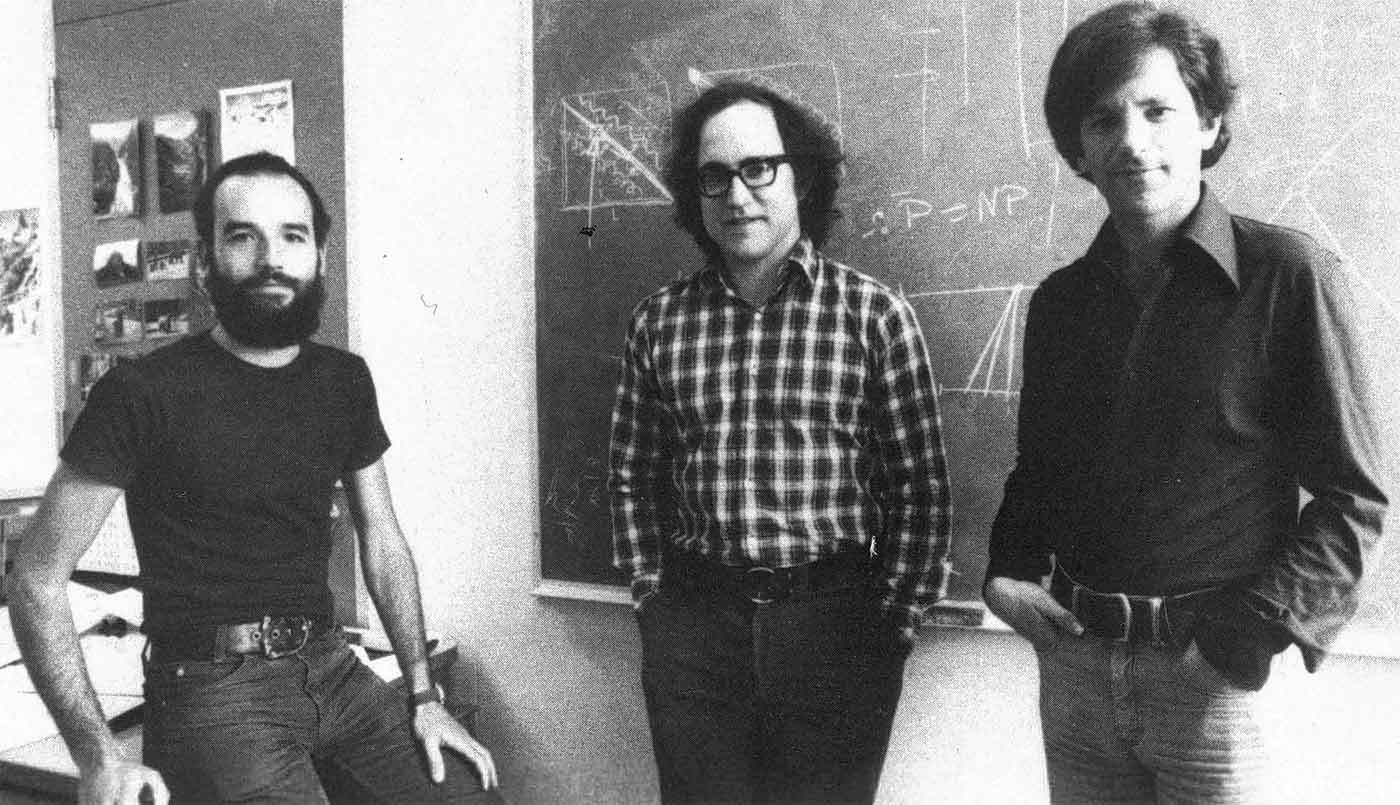
\includegraphics[scale=0.2]{rsa.jpg}
		\caption{Rivest, Shamir, Adleman at MIT}
		\label{fig:rsa}
	\end{figure}
\end{frame}

\subsection{Generating Keys}
\subsection{Encryption and Decryption}

\section{Proof of Correctness}
\subsection{Fermat's Little Theorem}
\subsection{Euler's Theorem}
\begin{frame}
	hello
\end{frame}

\end{document}
